% Extracted from reviewOfFamousFunctions.tex, problem #1
\begin{problem}
The graph of $g(x)=e^x$ is given below.

%	\begin{image}		
%	\includegraphics[scale=.6]{Figure1.pdf}
%	\end{image}	
	  \begin{center}
		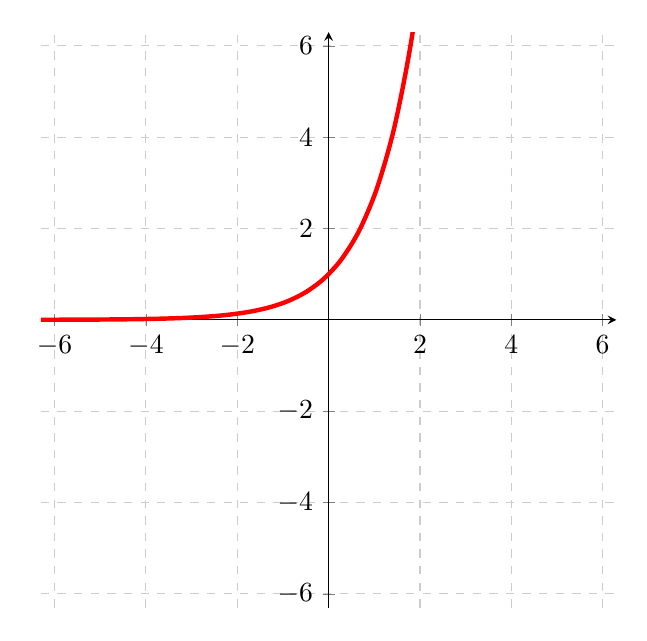
\begin{tikzpicture}
			\begin{axis}[
				xmin=-6.3, xmax=6.3, ymin=-6.3,ymax=6.3,    
				axis lines =middle, 
				every axis y label/.style={at=(current axis.above origin),anchor=south},
				every axis x label/.style={at=(current axis.right of origin),anchor=west},
				xtick={-6,-4,...,6}, ytick={-6,-4,...,6},
				grid=major, width=3.5in, height = 3.5in,
				grid style={dashed, gray!40}
				]
				\addplot[color=red, ultra thick, smooth, domain=-6.3:3]{exp(x)};				

			\end{axis}
		\end{tikzpicture}
	\end{center}
			

\begin{enumerate}	
	\item  Find the domain and range of $g$.
\WkstHop
		\begin{freeResponse}
			Domain: $(-\infty,\infty)$, Range: $(0,\infty)$
		\end{freeResponse}


	
	\item  Find the values of $g(1), g(0), g(-1)$ and plot the points $(1,g(1)), (0,g(0)),$ and $(-1,g(-1))$  on the graph of $g(x)=e^x$.
\WkstHop
		\begin{freeResponse}	
			$g(1)=e^1=e$ , $ g(0)=e^0=1$, and $g(-1)=e^{-1}=\frac{1}{e}$.
			 These are standard values of the famous function $g(x)=e^x$ that you should know.
		\begin{image}		
		\includegraphics[scale=.6]{Figure5.pdf}
		\end{image}


		\end{freeResponse}

	\item Graph $h(x)=\ln(x)$ on the same axis as $g(x)=e^x$.
\WkstHop
		\begin{freeResponse}
		Recall:  $\ln(x)$ is the inverse of $e^x$.  To find the graph of $\ln(x)$ we reflect the graph of $e^x$ over the line $y=x$.  Since the points $\left(-1,\frac{1}{e}\right),(0,1),(1,e)$ are on $y=e^x=g(x)$, the points $\left(\frac{1}{e}, -1\right),(1,0),(e,1)$ are on the graph of $y=\ln(x)=g^{-1}(x)=h(x)$ 

		\begin{image}		
		\includegraphics[scale=.7]{Figure4.pdf}
		\end{image}
		  \begin{center}
		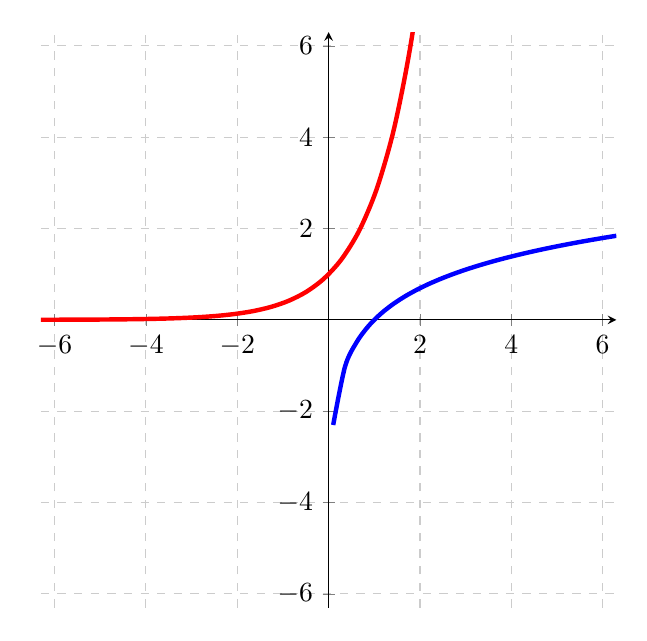
\begin{tikzpicture}
			\begin{axis}[
				xmin=-6.3, xmax=6.3, ymin=-6.3,ymax=6.3,    
				axis lines =middle, 
				every axis y label/.style={at=(current axis.above origin),anchor=south},
				every axis x label/.style={at=(current axis.right of origin),anchor=west},
				xtick={-6,-4,...,6}, ytick={-6,-4,...,6},
				grid=major, width=3.5in, height = 3.5in,
				grid style={dashed, gray!40}
				]
				\addplot[color=red, ultra thick, smooth, domain=-6.3:3]{exp(x)};				
				\addplot[color=blue, ultra thick, smooth, domain=0.1:6.3]{ln(x)};				
			\end{axis}
		\end{tikzpicture}
	\end{center}	
		\end{freeResponse}

	\item Find the domain and range of $h$.
\WkstHop
		\begin{freeResponse}
		The domain of $h(x)=\ln(x)$ is $(0,\infty)$.  The range is $(-\infty,\infty)$.
		\end{freeResponse}

	\item Find the values of $h(1), h(0), h(-1), h(e), h\left(\frac{1}{e}\right)$, or say $x$ not in the domain.
\WkstHop
			\begin{freeResponse}
			 $h(1)=\ln(1)=0$, $h(0)$ is not defined because $0$ is not in the domain of $\ln(x)$.
			$ h(-1)$ is not defined because $-1$ is not in the domain of $\ln(x)$.
			$h(e)=\ln(e)=1$, and $h\left(\frac{1}{e}\right)=\ln\left(\frac{1}{e}\right)=\ln\left(e^{-1}\right)= -1\ln(e)=-1$.
			 These are standard values of the famous function $h(x)=\ln(x)$ that you should know.
		\end{freeResponse}
	\end{enumerate}
	
 		
		
	
\end{problem}
